

\section{\tc Protocol}

We now describe the operation of \tc at the protocol level. The basic protocol is conceptually simple: A user contract \reqcont requests a datagram from the \tcontract \tcont. \tcont forwards the request to \engine and then returns the request to \reqcont. There are many details, however, relating to message contents and protection and the need to connect the off-chain parts of \tc with the blockchain.

First, we give a brief protocol overview. Then we enumerate the data flows in \tc. Finally, we provide a component-level view of the protocol by specifying the functionalities embodied in the \tcontract, \medname, and \encname. We present these  as ideal functionalities, inspired by the universal-composability (UC) framework, in order to abstract away implementation details and as a springboard for formal proofs of security. We omit details in this section on how payment is incorporated into \tc; this delicate aspect of the system design is deferred to Section~\ref{}.

\subsection{Datagram lifecycle}

The lifecycle of a datagram may be briefly summarized in the following steps:

\begin{itemize}
\item {\bf Initiate request.} \reqcont sends a datagram request to \tcont on the blockchain.

\item {\bf Monitor and relay.} The \medname monitors \tcont and relays any incoming datagram request with parameters \dgform to the \encname.

\item {\bf Securely fetch feed.} To process the request specified in \dgform, the \encname contacts a data source via HTTPS and obtains the requested datagram. It forwards the datagram via the Relay to \tcont.

\item {\bf Return datagram.} \tcont returns the datagram to \reqcont.
\end{itemize}

We now make this data flow more precise. 

\subsection{Data flows}

A datagram request by \reqcont takes the form of a message $m_1 = (\{\dgid\}, \dgform, \dgcallback)$ to \tcont on the blockchain. 
Here, $\dgid$ denotes a unique request identifier, as a technical matter assigned by \tcont to a message $(\dgcallback, \dgform)$ sent by \reqcont and communicated to \reqcont.  For simplicity, and to emphasize that all message flows are tagged with $\dgid$ we just depict $\dgid$, notated by $\{\dgid\}$, as part of the communicated message, and give details on its assignment below.

The parameter $\dgcallback$ in $m_1$ specifies the entry point in \reqcont to which the datagram is to be returned. (In principle, $\dgcallback$ could specify an entry point in a different contract, but \tc does not yet adopt this generalization.) $\dgform$ specifies the requested datagram, e.g., ${\sf params} := (\weburl, {\sf spec}, T)$, where $\weburl$ is the target data source and {\sf spec} specifies content of a the datagram to be retrieved (e.g., a stock ticker at a particular time), while $T$ specifies the delivery time for the datagram. 

\tcont forwards $m_2 = (\dgid, \dgform)$ to the \encname. It receives in return a return message $m_3 = (\dgid, \dgform, \dgm)$ from the $\tc$ service, where $\dgm$ is the datagram, i.e., contains the data (e.g., the desired stock ticker price). \tcont checks the consistency of $\dgform$ on the incoming and outgoing messages, and if they match forwards $\dgm$ to the entry point \dgcallback in \reqcont in message $m_4$. Finally, \reqcont uses $\dgid$ in $m_4$ to match the returned datagram to its original request.

Fig.~\ref{fig:dataflow} shows the data flows involved in processing a datagram request. For simplicity, the figure omits the \medname, which is only responsible for data passing.


%\begin{figure}[h!]
%\centering
%\begin{tikzpicture}
%  [entity/.style={rectangle,draw=black,minimum height=3em,text width=6em,align=center},
%   trusted/.style={fill=green!30},
%   communication/.style={blue,ultra thick,text=black},
%   bg-box/.style={rectangle,rounded corners,draw=black,dashed},
%   blockchain-color/.style={fill=yellow!20}]
%  \node[entity,trusted,minimum height=4.5em] (ctc) {};
%  \node[entity,draw=none,anchor=north] (ctc-inner) at (ctc.north) {TC Contract\\$\tcont$~~~~~};
%  \node[entity,trusted,right=7em of ctc] (enc) {Enclave};
%  \node[entity,fill=white,below=5em of ctc,anchor=north west,xshift=1em] (cu) {User Contract\\$\reqcont$};
%  \node[entity,trusted,minimum height=1.5em,text width=3em,anchor=south west] (id-gen) at (ctc.south west) {\footnotesize $\dgid$ gen};
%
%  \draw[-stealth,communication] ([yshift=-0.5em]cu.west) -| node [text width=3.3em,align=center,blockchain-color,yshift=3.5em] {\footnotesize $m_0 =$\\[-0.2em]$(\dgform,$\\[-0.2em]$\dgcallback)$} ([xshift=-2.4em]ctc.south);
%  \draw[-stealth,communication,thick,dashed] ([xshift=-0.5em]ctc.south) |- node [text width=3em,xshift=1.5em,xshift=0.5em,yshift=3em] {\footnotesize $m_1 =$\\[-0.2em]$(\dgid)$} ([yshift=0.5em]cu.west);
%  \path[-stealth,communication] (ctc) edge [above,transform canvas={yshift=0.6em}] node [text width=4em,align=center,xshift=-0.25em] {\footnotesize $m_2 =$\\[-0.4em]$(\dgid,\dgform)$} (enc);
%  \path[-stealth,communication] (enc) edge [below,transform canvas={yshift=-0.6em}] node [text width=4em,align=center] {\footnotesize $m_3 =$\\[-0.2em]$(\dgid,\dgform,$\\[-0.3em]$\dgm)$} (ctc);
%  \draw[-stealth,communication] ([yshift=-1.75em]ctc.east) -| node [text width=3em,align=center,blockchain-color,yshift=-3em] {\footnotesize $m_4 =$\\[-0.4em]$(\dgid,\dgm)$} (cu);
%
%  \path[-stealth,green!40!black,text=black,ultra thick] ($(id-gen.east)+(-0.25em,0)$) edge [above right] node [xshift=0.25em,yshift=0.25em] {\footnotesize $\dgid$} ($(id-gen.east)+(1em,1em)$);
%
%  \begin{pgfonlayer}{background}
%    \node[bg-box,
%          blockchain-color,
%          fit={($(ctc.north west)+(-0.75em,0.25em)$)($(cu.south east)+(0.75em,-0.25em)$)},
%          label=above:{\bf Blockchain}] (bc-bg) {};
%    \node[bg-box,
%          fill=black!20,
%          fit={($(enc.north east)+(0.5em,1em)$)($(enc.south west)+(-0.5em,-1em)$)},
%          label=above:{\bf TC Server}] (tc-bg) {};
%  \end{pgfonlayer}
%  \node[below=0.4em of tc-bg,align=center] (data) {\small (obtains $\dgm$\\from data source)};
%\end{tikzpicture}
%\caption{{\bf Data flows in datagram processing.}}
%\label{fig:dataflow}
%\end{figure}

\begin{figure}[h!]
\centering
\begin{tikzpicture}
  [entity/.style={rectangle,draw=black,minimum height=3em,text width=6em,align=center},
   trusted/.style={fill=green!30},
   communication/.style={blue,ultra thick,text=black},
   bg-box/.style={rectangle,rounded corners,draw=black,dashed},
   blockchain-color/.style={fill=yellow!20}]
  \node[entity,trusted] (ctc) {};
  \node[entity,draw=none,anchor=north] (ctc-inner) at (ctc.north) {TC Contract\\$\tcont$};
  \node[entity,trusted,right=7em of ctc] (enc) {Enclave};
  \node[entity,fill=white,below=5em of ctc] (cu) {User Contract\\$\reqcont$};
  \node[below=1em of enc,align=center] (data) {\small (obtains $\dgm$\\from data source)};

  \path[-stealth,communication] (cu) edge [transform canvas={xshift=-1.75em}] node [text width=3.5em,align=center,blockchain-color] {\footnotesize $m_1 =$\\[-0.2em]$(\dgform,$\\[-0.4em]$\dgcallback)$} (ctc);
  \path[-stealth,communication] (ctc) edge [above,transform canvas={yshift=0.6em}] node [text width=4em,align=center] {\footnotesize $m_2 =$\\[-0.4em]$(\dgid,\dgform)$} (enc);
  \path[-stealth,communication] (enc) edge [below,transform canvas={yshift=-0.6em}] node [text width=4em,align=center] {\footnotesize $m_3 =$\\[-0.2em]$(\dgid,\dgform,$\\[-0.4em]$\dgm)$} (ctc);
  \path[-stealth,communication] (ctc) edge [transform canvas={xshift=1.75em}] node [text width=2.5em,align=center,blockchain-color] {\footnotesize $m_4 =$\\[-0.4em]$(\dgm)$} (cu);

  \begin{pgfonlayer}{background}
    \node[bg-box,
          blockchain-color,
          fit={($(ctc.north west)+(-0.6em,0.3em)$)($(cu.south east)+(0.6em,-0.3em)$)},
          label=above:{\bf Blockchain}] () {};
    \node[bg-box,
          fill=black!20,
          fit={($(enc.north east)+(0.6em,0.3em)$)($(enc.south west)+(-0.6em,-0.3em)$)},
          label=above:{\bf TC Server}] () {};
  \end{pgfonlayer}
\end{tikzpicture}
\caption{{\bf Data flows in datagram processing.}}
\label{fig:dataflow}
\end{figure}


%\begin{figure}[h!]
%\centering
%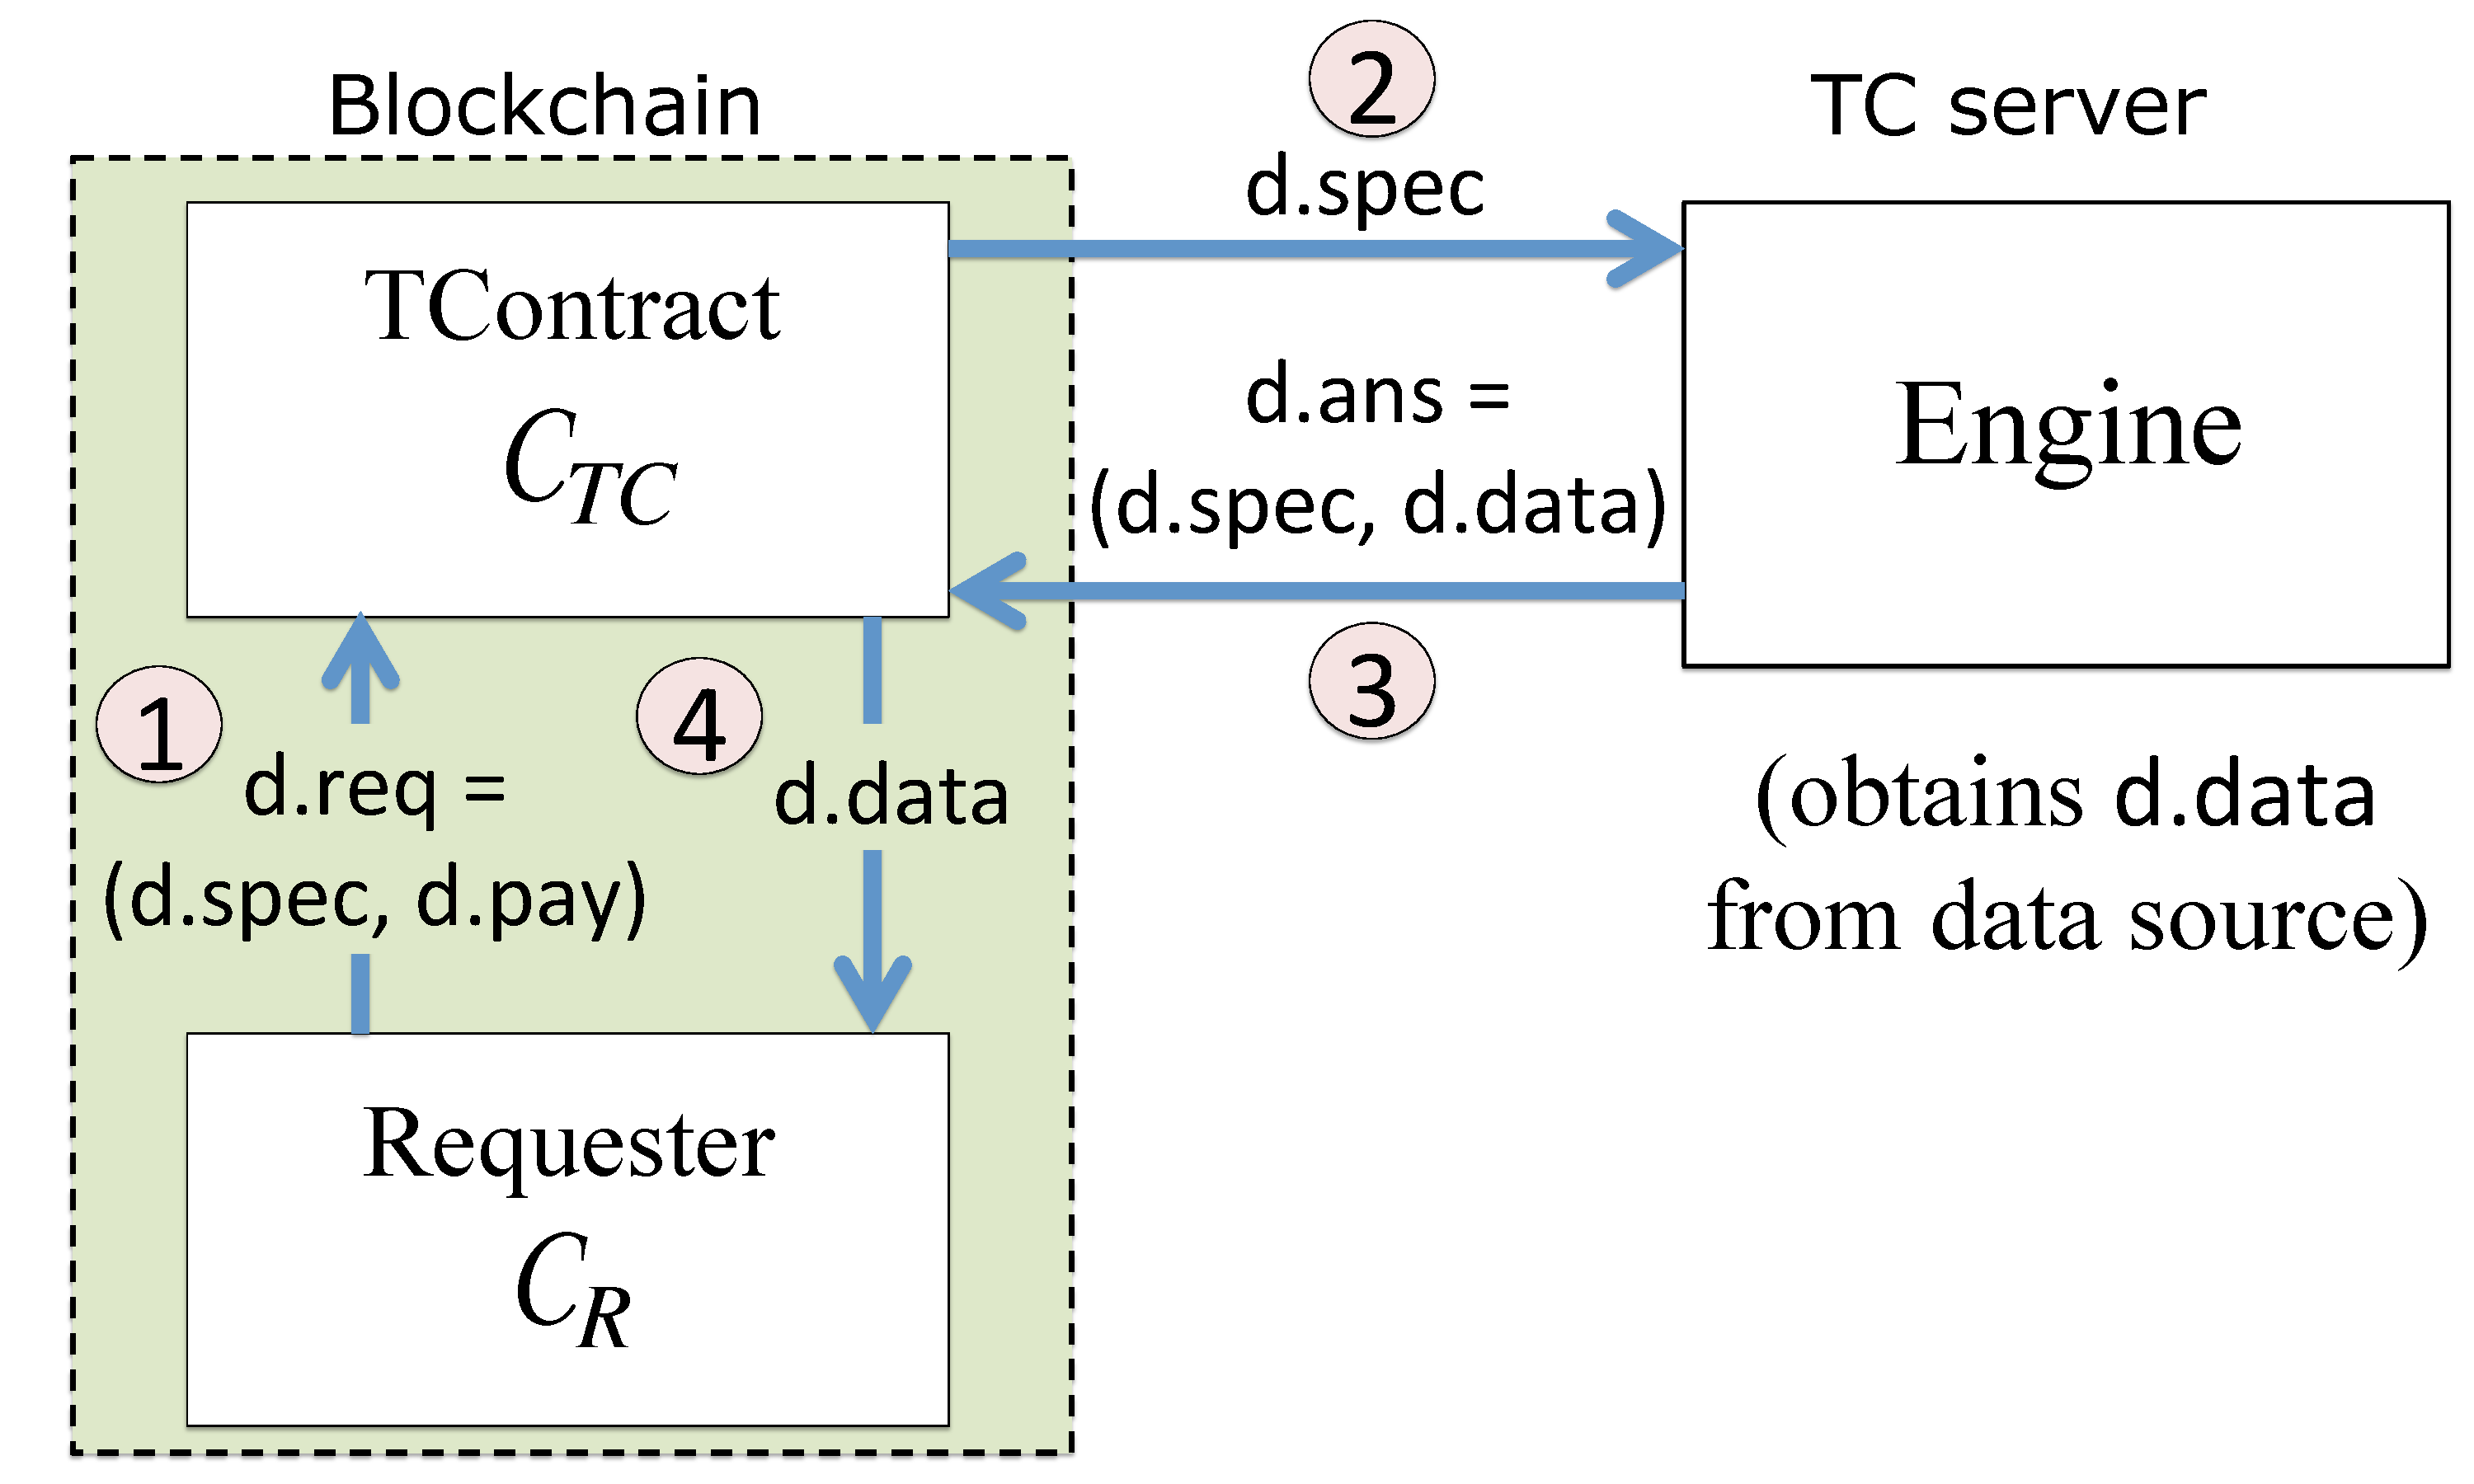
\includegraphics[width=\columnwidth]{figures/DataflowFig}
%\caption{{\bf Data flows in datagram processing.} \elaine{the figure must be changed,
%  m1 and m4 do not have id in the formal algorithm descriptions} }
%\label{fig:dataflow}
%\end{figure}


Digital signatures are needed to authenticate messages, such as $m_3$, entering the blockchain from an external source. We let $(\skTC, \pkTC)$ denote the private / public keypair associated with the \encname for such message authentication. For simplicity, Fig.~\ref{fig:dataflow} assumes that the \encname can send signed messages directly to \tcont. We explain shortly how Ethereum requires a slightly different approach in which \tc sends messages via an Ethereum wallet \tcadd.


\subsection{Use of SGX}

Let $\enclaveprog$ represent the code for \encname, which we presume is trusted by all system participants. Our protocols in \tc rely on the ability of SGX to attest to execution of an instance of $\enclaveprog$ and bind a public key $\pkTC$ to this instance. Here we briefly explain how we achieve these goals. First, we present a model that abstracts away implementation details in SGX and helps simplify our protocol presentation and later, our security proofs. \ari{Cite Elaine's SGX paper.} We then explain how SGX attestation is used to authenticate datagrams served by \tcont, namely through binding of $\pkTC$ to an Ethereum wallet on the blockchain. Finally, we explain how we use the clock in SGX.



\paragraph{\bf Formal model and notation.} 

We abstract away details of the functioning of SGX in two ways.
First, we abstract away the use of group signatures in EPID and simply denote the keypair associated with group signatures for all legitimate SGX hosts by $(\pkM, \skM)$. 
We let $\Sigma.{\sf Sign}({\sk}, X)$ denote a digital signature under private key $\sk$ of message $X$, and $\Sigma.{\sf Verify}({\sk}, \sigma, X)$ denote the corresponding verification operation. 

Second, we model execution in SGX in terms of a functionality $\fsgx$ operating in a stateful manner on \enclaveprog, and specified in Figure~\ref{fig:SGX_abstraction}. $\fsgx$ may be be invoked with one of two messages to \enclaveprog: \initcall, which creates the enclave with \enclaveprog as its initial state and triggers measurement quotes and (\resumecall, $X$) which initiates an execution of \enclaveprog on a fresh input $X$. (We assume that \enclaveprog exits only when it completes processing of a given input.) We let $\fsgx[\enclaveprog, \relay]$ denote invocation of $\fsgx$ on \enclaveprog by \relay. 


\begin{figure}[ht!]
\begin{boxedminipage}{\columnwidth}
\begin{center}
{\bf $\fsgx[\enclaveprog, \relay]$: abstraction for SGX}
\end{center}
\begin{tabular}{l}
{\bf Hardcoded:} $\skM$ \\[5pt]

{\bf Assume:} \\ 
$\enclaveprog$ has entry points {\bf Initialize} and {\bf Resume}\\[5pt]

{\bf Initialize:}\\
On receive ``initialize'' from $\relay$: \\
\quad Let ${\sf outp} := \enclaveprog.{\bf Initalize}()$  \\
\quad $\sigatt := \sigsgx.{\sf Sign}(\skM, (\enclaveprog, {\sf outp}))$ \\[-1pt]
\qquad \qquad {\it //~models EPID sig.}\\
\quad Output  $({\sf outp}, \sigatt)$\\[5pt]

On receive (``resume'', ${\sf params}$) from $\relay$: \\
\quad Let ${\sf outp} := \enclaveprog.{\bf Resume}({\sf params})$  \\
\quad Output ${\sf outp}$ 
\end{tabular}
\end{boxedminipage}
\caption{Formal abstraction for SGX execution capturing a subset of SGX features
sufficient for implementation of \tc.
}
\label{fig:SGX_abstraction}
\end{figure}


\paragraph{Binding $\enclaveprog$ to Ethereum wallet \tcadd.}
Information can only be inserted into the blockchain in Ethereum as a transaction from a wallet. Thus, the only way the \medname can relay messages form the \encname to \tcont is through a wallet (again, formally, an externally owned account) \tcadd. Since the \medname may corrupt messages, however, it is critical that they be authenticated by the \encname. Since Ethereum itself 
already verifies signatures on transactions from externally owned accounts (i.e., users interact with the  Ethereum blockchain through an authenticated channel), \tc uses a trick to {\it piggyback verification of enclave signatures on top of Ethereum's already existing transaction signature verification mechanism}. 

Very simply, the \encname creates \tcadd with the public key \pkTC. 

To make this idea work fully, the public key $\pkTC$ must be hardcoded into \tcont. A client creating or relying on a contract that uses \tcont is responsible for making sure that this hardcoded $\pkTC$ has an appropriate SGX attestation before interacting with the $\tcont$  blockchain contract.  Let {\sf Verify} denote a verification algorithm for EPID signatures. Fig.~\ref{fig:att_check} gives the protocol for a client to check that \tcont is backed by a valid \encname instance. This protocol does not include a mechanism for \emph{revocation} of a compromised SGX instance, an issue we discuss later in the paper.

In summary, then, we may assume in our protocol specifications that {\em all relying clients have verified an attestation for \encname and thus that datagram responses passed from \tcadd to \tcont are trusted to originate from \engine.} 



\begin{figure}[htb!]
\begin{boxedminipage}{\columnwidth}
\begin{center}
{\bf User: offline verification of SGX attestation}
\end{center}
\begin{tabular}{l}
{\bf Inputs}: $\pkM$, $\pkTC$, $\enclaveprog$, $\sigatt$ \\[5pt]
{\bf Checks:} \\
Assert $\enclaveprog$ is the expected enclave code\\
Assert $\sigsgx.{\sf Verify}(\pkM, \sigatt, (\enclaveprog, \pkTC))$ \\
Assert \tcont is correct and parametrized w/ \pkTC\\
{\it //~now okay to rely on \tcont}
\end{tabular}
\end{boxedminipage}
\caption{A client checks an SGX attestation on the enclave's code $\enclaveprog$ and public key $\pkTC$; the client
checks that $\pkTC$ is hardcoded into \tc blockchain contract \tcont before 
using \tcont.
} 
\label{fig:att_check}
\end{figure}



\paragraph{\bf SGX Clock.}
As noted above, trusted clock provides only relative time with respect to a reference point, not absolute time. Thus, when initialized, the \encname is provided with the current wall-clock time by a trusted source, e.g., the \medname (under a trust-on-first-use model). In the current implementation of \tc, clients may request via a web interface in the \medname a fresh timestamp, signed by the \encname under \pkTC, that clients may verify in real time. Thus, a client can determine the absolute clock time of \encname to within a high degree of accuracy, bounded by the round-trip time of its attestation request plus the attestation verification time--on the order of hundreds of milliseconds in a wide-area network~\cite{}. A high degree of accuracy is potentially useful for some applications but only loose accuracy is not required for most. Ethereum has a block interval of 12s and the clock serves in \tc primarily to: (1) Schedule connections to data sources and (2) To check TLS certificates for expiration when establishing HTTPS connections. For simplicity, we just assume in our protocol specifications that the \encname clock provides accurate wall-clock time (in the canonical format of seconds since the Unix epoch January 1, 1970 00:00 UTC).

We let $\clock()$ denote measurement of the SGX clock from within the enclave; $\clock()$ returns the current absolute (wall-clock) time. 


\subsection{A payment-free basic protocol}
For simplicity, we first specify a payment-free version of our basic protocol, i.e., one that does not include gas or fees. Later, in our implementation discussion, we explain how we handle these two resources, and we prove payment-related properties in the paper appendix. For simplicity, we assume a single instance of \engine, although our architecture could scale up to multiple enclave and even server instances. To show messages corresponding to those in Fig.~\ref{fig:dataflow}, we use the label ({\bf msg.}~$m_i$)

\paragraph{The Requester Contract $\reqcont$.}
The requester contract $\reqcont$ sends to the \tcontract \tcont
a request of the form $(\dgform, \dgcallback)$.
%which \tcont converts into a message $m_1 = (\dgform, \dgcallback)$ as specified below.

\paragraph{The \tcontract \tcont.} 
The \tcontract, as noted above, accepts a datagram request from \reqcont, 
assigns a unique ${\sf id}$ to each request, and
records the request.
%\tcont
%now
%forwards the request to the \tc server, and 
Our Town Crier Relay $\relay$ will monitor
requests received by \tcont, and 
forwards the requests to an SGX enclave.
When $\tcont$ obtains a valid response
from $\tcadd$,   
it 
sends the resulting datagram $\dgm$ to the entry point \dgcallback 
specified by the requesting contract \reqcont. As explained above, because the response (msg. $m_2$) comes from $\tcadd$, the blockchain automatically verifies that the response is correctly signed under $\engine$'s key $\pkTC$, and \tcont need not verify the signature explicitly. \tc does, however, have a subtle security requirement. Specifically,  for a given datagram request $\dgid$, \tcont must verify that $\dgform' = \dgform$, where $\dgform$ is the digitally signed message produced by \engine and $\dgform$ is the locally stored parameters. The check is necessary to prevent \relay from corrupting datagram requests passed by \tcont (which, as a public function, has no means of digitally signing requests). 

\tcont is specified in Fig.~\ref{fig:tc-contract}. Here, Call denotes a call to a contact entry point, while Return denotes a message returned by the blockchain in response to a function call. Counter is a variable such that Counter = 0 upon creation of \tcont.
\begin{figure}[!htb]
\begin{tabularx}{\linewidth}{|@{\hspace{3pt}}r@{\hspace{1ex}}X@{\hspace{3pt}}|}
  \hline

  \multicolumn{2}{|c|}{{\bf Program for Town Crier blockchain contract \tcont}} \\ [1ex]
{\bf Initialize:} &  Counter := 0\\
  {\bf Request:} & On recv $(\dgform, \dgcallback)$ from some $\reqcont$:   
 \\
%                 & If $(\${\sf fee} < F_{\rm min}$ or $\${\sf fee} > F_{\rm max})$ \\
%                 & \hspace*{1em} Return $\${\sf fee}$ to $\pkU$ \\

		& \dgid :=  Counter; \ \ Counter := Counter + 1 \\
%		& Return(\dgid) \\
                 & Record $(\dgid, \dgform, \dgcallback)$ 
\quad {\sgray{\it //~{\bf msg.}~$m_1$}} 
\\
 		& Return $\dgid$
\\[5pt] 
%		 & Send $(\dgid, \dgform)$ to \relay \\
%\multicolumn{2}{|c|}{\sgray {\it // above implemented by \relay monitoring the blockchain}}\\[5pt]
  {\bf Deliver:} & On recv $(\dgid, \dgform, \dgm)$ from $\tcadd$: \\
		 & Retrieve recorded $(\dgid, \dgform', \dgcallback)$\\
		 & Assert $\dgform = \dgform'$\\
                 & Call ${\dgcallback}({\dgm})$ \quad \sgray{\it //~{\bf msg.}~$m_4$}\\
%                 & Send $\${\sf fee}$ ether to $\Psgx$. \\

  \hline
\end{tabularx}
\caption{
The Town Crier \tcontract \tcont.
}
\label{fig:tc-contract}
\end{figure}

\paragraph{The \encname \engine.} When initialized through an \initcall call, \engine sets its absolute clock (by setting a reference point) and generates a keypair $(\pkTC,\skTC)$ to which it binds by placing $\pkTC$ in attestation requests. Given input \resumecall $({\sf id}, {\sf params})$, \engine contacts the requested data source via HTTPS and checks that the corresponding certificate {\sf cert} is valid, i.e., not expired. We defer discussion of certificate revocation to Section~\ref{}. \engine then fetches the requested datagram and returns it to \relay along with the inputs, all digitally signed. The protocol for \engine is shown in Fig.~\ref{fig:engineprotocol}.

\begin{figure}[!h]
\begin{boxedminipage}{\columnwidth}
\begin{center}
{\bf Program for \tcs~\encname ($\enclaveprog$)}
\end{center}
\begin{tabular}{l} 
{\bf Initialize}:  On recv (\initcall): \\ %{\it //~called only once upfront}\\
%\quad Set clock reference point\\
%\quad Record $T_0$ \elaine{this is never used} \\ 
%\elaine{i deleted the clock implementation, we can separate abstraction from implementation.}\\
\quad $(\pkTC, \skTC) := \Sigma.{\sf KeyGen}(1^\lambda)$\\
%\quad Record $(\pkTC, \skTC)$\\
\quad Output $\pkTC$   \\
\sgray{\it/* Subroutine call from $\fsgx$, which attests to}\\ 
\quad \sgray{\it$\enclaveprog$ and $\pkTC$.} 
 \sgray{See Figure~\ref{fig:SGX_abstraction}.*/}
\\[3pt]

%{\bf Attest}:  On recv \attcall: \\ %{\it //~called only once upfront}\\
%\quad $T := \clock()$\\
%\quad Call quoting enclave with supp.~data $(\pkTC, T)$
%\\[5pt]

{\bf Resume:} On recv (\resumecall, $({\sf id}, {\sf params}))$\\
\quad Parse ${\sf params} := (\weburl, \dgspec, T) $:\\
\quad Assert $\clock() \geq T$\\
\quad Contact $\weburl$ via HTTPS, obtaining ${\sf cert}$ \\
\quad Verify {\sf cert} is valid for time $\clock()$\\
\quad Obtain webpage $w$ from $\weburl$ \\
\quad Parse $w$ to extract \dgm with specification (\dgspec, $T$) \\
\quad $\sigma := \Sigma.{\sf Sign}({\skTC}, ({\sf id}, {\sf params}, {\sf data}))$\\
\quad Output $(({\sf id}, {\sf params}, {\sf data}), \sigma)$
\end{tabular}
\end{boxedminipage}
\caption{
The \tcs~\encname \engine.
} 
\label{fig:engineprotocol}
\end{figure}

\paragraph{The \medname \relay.} As noted in Section~\ref{sec:architecture}, \relay performs distinct three forms of data passing, which we  specify more precisely here. It scrapes the blockchain, monitoring \tcont for new datagram requests $({\sf id}, {\sf params})$. It boots the \engine with an \initcall call and handles incoming requests by invoking \engine with a \resumecall call. Finally, it forwards datagram responses from \engine to the blockchain; recall that it inserts data onto the blockchain and thus forward responses through \tcadd. The program for \relay is shown in Fig.~\ref{fig:relayprotocol}. Here, the function AuthSend denotes a blockchain transaction (sent from $\tcadd$ signed with $\skTC$).

\begin{figure}[!h]
\begin{boxedminipage}{\columnwidth}
\begin{center}
{\bf Program for Town Crier \medname $\relay$}
\end{center}
\begin{tabular}{l}
{\bf Initialize}:\\
Send \initcall to $\fsgx[\enclaveprog, \relay]$\\
On recv $(\pkTC, \sigatt)$ from $\fsgx[\enclaveprog, \relay]$:\\
\quad Publish $(\pkTC, \sigatt)$\\[5pt]

{\bf  Loop forever}: \\
%{\bf Request}:
Whenever \tcont records 
a request
$({\sf id}, {\sf params}, \_)$:  \\  %\sgray{{\it //~{\bf msg.}~$m_2$}}\\
\quad Parse ${\sf params} := (\weburl, \dgspec, T)$\\
\quad {\bf Fork}: \\
\ \quad Wait until $\clock() \geq T$\\
\ \quad Send $(\text{\resumecall}, ({\sf id}, {\sf params}))$ to $\fsgx[\enclaveprog, \relay]$ \\
\ \quad On recv $(({\sf id}, {\sf params}, {\sf data}), \sigma)$ from $\fsgx[\enclaveprog, \relay]$:\\ 
\ \quad \quad  {\sf AuthSend} $({\sf id}, {\sf params}, {\sf data})$ to \tcont as \tcadd \\
\hspace{50mm}\sgray{\it //~{\bf msg.}~$m_3$}\\
\end{tabular}
\end{boxedminipage}
\caption{The Town Crier \medname \relay.}
\label{fig:relayprotocol}
\end{figure}


